\chapter{Background}
\label{ch:background}


% \sweExpl{Bakgrund}
% \generalExpl{When you do your literature study, you should have a nearly complete Chapters 1 and 2.\\
% You may also find it convenient to introduce the future work section into your report early – so that you can put things that you think about but decide not to do now into this section.\\
% Note that later you can move things between this future work section and what you have done as you may change your mind about what to do now versus what to put off to future work.
% }
% \generalExpl{What does a reader (another x student -- where x is your study line) need to know to understand your report?
% What have others already done? (This is the “related work”.) Explain what and
% how prior work/prior research will be applied on or used in the degree
% project/work (described in this thesis). Explain why and what is not used in
% the degree project and give valid reasons for rejecting the work/research.}


This chapter provides the necessary background for understanding the research conducted within this thesis. This chapter also showcase the related work for this thesis and how the research relates to it.


% \sweExpl{Vilken viktig litteratur och
% (forsknings-)artiklar har du studerat inom området (litteraturstudie)? }


\section{Neural Networks}


Neural network models are a type of models within the broader field of machine learning whose design have been inspired by human brains. These models allow computers to recognise patterns and solve complex problems. The backpropagation algorithm was popularised by Rumelhart, Hinton, and Williams \cite{rumelhart_learning_1986}. This algorithm efficiently computes the gradient of the loss function with respect to the weights of the network by propagating the error back from the output layer to the input layer. This method is critical to understand all machine learning pipelines because it enables the network to adjust its weights in a way that minimises the error, thereby improving the model's predictions over time.


Building on backpropagation, Yann LeCun et al. \cite{lecun_gradient-based_1998} introduced the \gls{CNN} architecture in 1998. These are a specialised kind of neural network for processing data, such as images, which can be converted to a matrix. \gls{CNN}s utilise layers with convolving filters that apply the learned weights across subsections of the input data. This reduces the amount of parameters in the network and improves its efficiency.


These are two steps in the evolution of neural network models, particularly the developments in \gls{CNN}s and other deep learning technologies, are central for setting the stage for even more complex architectures aimed at processing not just visual data, but sequential data such as text. This will eventually lead to Large Language Models (\gls{LLM}), which leverage deep learning techniques to understand and \textit{generate} human language. \gls{LLM}s are built upon the principles of neural networks. Understanding the models we commonly refer to as \gls{LLM}s involves understanding models such as Transformer models, \gls{BERT}, and other encoder-decoder networks.


\subsection{Recurrent Neural Networks (RNNs)}


A Recurrent Neural Network (\gls{RNN}) is a type of neural network that is good for modelling sequential data. They are significantly different from other neural networks in their ability to maintain memory of previous inputs using an internal state. This state which is maintained inside the network while it’s running, will influence the network’s output. \gls{RNN}s proved to be fundamental in tasks where context was crucial, such as language modelling and generation of text.


In an \gls{RNN}, each neuron, its most basic building block, processes a part of the sequence, receiving both the current input \(x_t\) and the output from the previous step \(h_{t-1}\), this is known as the "hidden state". The core of an \gls{RNN} operation involves updating this hidden state using:
\[
h_t = \text{tanh}(W_{hh} h_{t-1} + W_{xh} x_t + b)
\]
where \(W_{hh}\) and \(W_{xh}\) are the weights for the hidden state and input, respectively, and \(b\) is a bias. The updated state \(h_t\) is used in the next step to generate the output \(y_t\) via:
\[
y_t = W_{hy} h_t + b_y
\]




However, \gls{RNN}s often struggle with maintaining a longer context due to problems like vanishing and exploding gradients, as written by Hochreiter and Schmidhuber \cite{hochreiter_long_1997}. This was a problem other \gls{RNN} models tried to mitigate as it significantly reduce their usefulness in various tasks. The vanishing gradient problem makes it difficult for the \gls{RNN} to learn connections between events that occur at longer distances in the input sequence because the gradient of the loss function decays exponentially with the length of the input sequence.


This led to the development of more sophisticated variants like \gls{LSTM} networks and \gls{GRU}s were developed. \gls{LSTM}s \cite{hochreiter_long_1997}, use input, output, and "forget gates" to manage information flow, which allows them to maintain stable gradients. \gls{GRU}s, which was proposed by Cho et al. \cite{cho_learning_2014}, simplifies this by merging the gates and states, reducing complexity while preserving performance across various tasks.


\subsection{Sequence-to-Sequence Models}


\gls{seq2seq} models are designed to process sequences of data, such as text or speech, and generate corresponding output sequences. Sutskever et al. \cite{sutskever_sequence_2014} were the first to introduce these models which typically consist of two main components: an encoder and a decoder. The encoder will process the input and convert it into a dense vector. This vector encodes the entire input sequence which is then passed to the decoder, which generates the output. This architecture proved very useful in certain tasks such as translating text between languages. Bahdanau, Cho, and Bengio built upon this concept with attention mechanisms \cite{bahdanau_neural_2016} which would allow the decoder to focus on a specific piece of the input for small parts of the output, which improved the models ability to focus on longer sequences.


\subsection{Transformer Models}


The Transformer model, introduced by Vaswani et al. \cite{vaswani_attention_2023}, was a new approach for \gls{seq2seq} networks, with a self-attention mechanism which was different from the recurrent design of \gls{RNN}s. The new transformer architecture introduced by Vaswani et al. allowed the network to weigh the importance of different tokens in the input data irrespective of their sequential position. Where a token is a sequence of characters that can be treated as a single logical entity in the input and output sequence.


The key innovation of the Transformer is its ability to handle dependencies between single tokens or sequences of tokens at long distances from each other. This makes the transformer architecture especially good at understanding context in text data.


The introduction of the transformer model was foundational in the field, and today most models use this architecture, see section~\ref{sec:openai_models} and ~\ref{sec:mistral_models}.


\subsection{BERT and Advances in Encoder-Decoder Models}
\label{sec:bert_and_encoder_decoder}


\gls{BERT} was introduced by Devlin et al. \cite{devlin_bert_2019} in 2018 and was a major improvement within natural language processing. The \gls{BERT} model optimised token representations bidirectionally which means that it was refining the understanding of each token by looking at the tokens before and after each token. \gls{BERT} was built on the transformer model’s encoder which allowed for pre-training on large text corpora, followed by fine-tuning for various tasks such as sentiment analysis and question answering.


Encoder-decoder models are important in machine learning for tasks that involve converting one sequence into another, such as machine translation or speech-to-text. In this type of model the encoder processes the input sequence and compresses information into what’s known as a context vector, this is a condensed representation of the input data. The decoder takes this context vector and generates an output sequence token by token. Each of these two components may be built using recurrent networks, convolutional networks, or more commonly nowadays, transformer architectures.


In contrast to traditional encoder-decoder models, encoder-only models, such as \gls{BERT}, focus on generating an output based on an input without the need for a decoder. These models are typically used for tasks that require deep understanding of language context like sentence classification.


Decoder-only models, like the \gls{GPT} (see section~\ref{sec:openai_models}), focus on generating sequences from a given context or starting point. These models are very good in situations where the model needs to exhibit "creative" properties, such as when generating text completions.


Parallel to \gls{BERT}, other encoder-decoder models like the Transformer \cite{vaswani_attention_2023} and \gls{seq2seq} networks with attention mechanisms \cite{bahdanau_neural_2016} have shown great results when translating sequences in tasks like machine translation, exemplified by Google's Neural Machine Translation system \cite{wu_googles_2016}, and speech recognition, as seen in Apple's Siri voice assistant \cite{hinton_deep_2012}.


\section{Generative AI}


Generative AI is a term used to describe a subset of artificial intelligence technologies that are designed to create new content. This can be images such as with DALL-E \cite{ramesh_zero-shot_2021}, text with models like GPT-3 \cite{brown_language_2020} or movies \cite{openai_video_2024}. These models are capable of generating realistic and arguably novel outputs by understanding and simulating the underlying structure of the training data. One of the most popular frameworks in Generative AI includes \gls{GAN}s, introduced by Goodfellow et al. \cite{goodfellow_generative_2014}, which consist of two neural networks, the generator and the discriminator. These two networks will compete against each other. The generator creates items that are as realistic as possible, and the discriminator evaluates them. This process runs until the discriminator can no longer accurately separate generated items from the training data.


\section{State-of-the-Art Large Language Models}


\gls{LLM} represent a significant breakthrough in \gls{NLP}. They are capable of understanding and generating text similar to that written by humans. In recent years, several cutting-edge \gls{LLM}s have been developed by prominent companies and research institutions that have gained wide-spread use. This section gives an overview of some notable examples of these advanced \gls{LLM}s.


\label{sec:openai_models}
\subsection{OpenAI's GPT Series}


OpenAI's \gls{GPT} series of language models have over the past few years featured some of the most widely used language models. GPT-1 was first released in 2017 followed by GPT-2, GPT-3, and GPT-4 (with various variants of these models). GPT-3, in particular, with its 175 billion parameters, has demonstrated strong capabilities in tasks such as text completion, question answering, and even code generation \cite{brown_language_2020}. These models are some of the most widely used models, primarily due to their popularisation by the product from the same company, ChatGPT \footnote{\href{https://chat.openai.com}{chat.openai.com}}.


\subsection{Mistral}
\label{sec:mistral_models}


Mistral is a french firm that has released a few models that has gained widespread adoption in the open source community. As of writing, \textit{Mistral-7B-Instruct-v0.2} had 2,297,845 million downloads on huggingface last month \footnote{\href{https://huggingface.co/mistralai/Mistral-7B-Instruct-v0.2}{The huggingface page for Mistral-7B-Instruct-v0.2}}, and Mixtral-8x7B-Instruct-v0.1 had 628,927 \footnote{\href{https://huggingface.co/mistralai/Mixtral-8x7B-Instruct-v0.1}{The huggingface page for Mixtral-8x7B-Instruct-v0.1}}.


\textit{Mistral 7B v0.1} \cite{jiang_mistral_2023} was their first major model to get widespread notoriety. The model is a 7-billion-parameter language model which was small enough to run on consumer-grade GPUs. The model utilised \gls{GQA}\cite{ainslie_gqa_2023} and \gls{SWA} \cite{roy_efficient_2020} techniques to achieve impressive results across various benchmarks, including reasoning, mathematics, and code generation tasks. \textit{Mistral 7B v0.1 instruct} is a related fine-tuned model.


The "instruct" version of generative AI models, such as the Mistral 7B, has been fine-tuned to follow prompted instructions. In contrast, the base model simply generates output based on the provided prompt. This process was first published by the team at OpenAI \cite{ouyang_training_2022}, however it’s also employed by mistral and other model vendors. This approach is commonly used for models deployed in AI assistants or chat applications.


The \textit{Mixtral of Experts} model \cite{jiang_mixtral_2024}, is a variant of the Mistral model that introduces a \gls{SMoE} architecture, as described by Jiang et al. \textit{Mixtral-8x7B-Instruct-v0.1} employs 8 feedforward blocks (experts) in each layer, with a router network selecting two experts for processing and combining their outputs at each timestep. The model has access to 47 billion parameters, but effectively only utilise 13 billion parameters during inference, which makes the model easier to deploy on GPUs with less amounts of memory.


\subsection{Google's Language Models}


Google has two major families of model, the first being the Gemini family, as introduced in a series of papers by Google's team \cite{gemini_team_gemini_2024-1}, consists of models like Gemini Ultra, Pro, and Nano, each of these models are designed for specific applications and more importantly size of GPU. Where the larger models require enterprise-grade GPUs that are expensive to operate. Gemini 1.5 extended on these models with an even larger context window by effectively processing and recalling information across millions of tokens in a multi-modal context (tokens include both text, audio and image tokens) \cite{gemini_team_gemini_2024}. This is the first model to demonstrate resilience to the problem first described by Nelson et al. where the model would be biassed towards instructions or data in the beginning and end of larger prompts \cite{liu_lost_2023}.


Goggles Gemma family of models \cite{gemma_team_gemma_2024} represents Google's effort to provide state-of-the-art, lightweight models to the open source community. These models, available in sizes of 2 billion and 7 billion parameters. The models demonstrate worse performance against their Gemini class of models across all tasks such language understanding and reasoning. However, the Gemma models’ size make them easier to deploy on smaller consumer-grade GPUs.


\subsection{The LLama family of models}


In February 2023, Meta AI released LLaMA \cite{touvron_llama_2023-1} in four distinct sizes: 7, 13, 33, and 65 billion parameters. The model utilised features such as SwiGLU activation functions, rotary positional embeddings, and root-mean-squared layer-normalisation to achieve comparable results to OpenAIs GPT-3 model. Despite being initially released under a noncommercial licence, the weights of LLaMA were leaked, prompting widespread unauthorised use. This accelerated its adoption across various applications.


Later in July of 2023, Meta released LLaMA-2 \cite{touvron_llama_2023-2} which was built upon the foundational models of its predecessor with enhanced data sets of 2 trillion tokens, fine-tuning capabilities, and improved dialogue system performance through specialised LLaMA-2 Chat models, these are similar to the instruct models mentioned in section ~\ref{sec:mistral_models}. LLaMA-2 had a 40\% larger training corpus and extended the context length to 4,000 tokens. The release included model sizes from 7 to 70 billion parameters. These models were released under a similar licence to the first LLaMA models.


Recently, in April 2024, Meta AI released LLaMA-3, this time with two models, one 8 billion parameter model and one 70 billion parameter model. These were open source and available online \footnote{\href{https://github.com/meta-llama/llama3}{The GitHub repository for LLaMA-3}} from day one under a commercial licence. The model was pre-trained on approximately 15 trillion tokens. Meta announced an, as of writing, future release of a 400 billion parameter model.


\subsection{Notable other vendors}


Besides the major players such as OpenAI, Google, and Meta, there exists a vast array of players, of varying size, that also develops language models. These include, but are not limited to, Anthropic, IBM and DeepMind (which is also a part of Google).


\section{Prompt engineering}
\label{sec:prompt_engineering}


Prompt engineering is the name given to the technique that evolved from the use of language models. This is the task of optimising the performance of a \gls{LLM} such as GPT-4, LLaMA, and others. This involves crafting the input text, or \textit{"prompt"} to these models in a way that guides them to produce desired outputs \cite{kathiriya_power_2023, chen_unleashing_2023}.


Prompt engineering is defined as the practice of designing input prompts that maximise the efficacy and accuracy of \gls{LLM} outputs. It is a key factor in the success of deploying \gls{LLM}-based applications. The process of prompt engineering involves several key techniques. A prompt should, according to Chen et al. include clear instructions and enough contextual details to guide the model towards providing the expected answer in the expected format. There are numerous advanced techniques such as "role-prompting", zero-shot, one-shot, and few-shot prompting that can improve the performance of \gls{LLM}.


For instance, Kathiriya et al. \cite{kathiriya_power_2023} demonstrates that role-prompting produces responses with heightened professional relevance. Similarly, Chen et al. highlight how few-shot prompting can refine the model's ability to perform complex analytical tasks by providing some targeted examples. Both of these studies show how prompt engineering techniques can improve performance.


Figure \ref{fig:role_prompt}, taken from the paper published by Chen et al. \cite{chen_unleashing_2023} illustrates an example of role-prompting. In this example the \gls{LLM} is instructed to assume the role of an expert in artificial intelligence, which aligns its responses with specific professional knowledge.


\begin{figure}[H]
\centering
\begin{tikzpicture}
    \newlength{\boxwidth}
    \setlength{\boxwidth}{0.4\textwidth}

    \node[draw, rectangle, rounded corners=2pt, inner sep=5pt, text width=\boxwidth, align=center] (a) {
        \smaller{You are an expert in artificial intelligence specialising in large language models...}
    };
    \node[draw, rectangle, rounded corners=2pt, inner sep=5pt, text width=\boxwidth, align=center, right=of a, xshift=0.5cm] (b) {
        \smaller{Here are five basic methods to quickly get started with large language models: \\\\ 1. Experiment with web-based interfaces \\\\ ...}
    };

    \draw[-latex, line width=1mm] (a) -- (b);

    \node[align=center, below=0.1cm of a] (c) {\footnotesize A role prompt};
    \node[align=center, below=0.1cm of b] (d) {\footnotesize Model output};
\end{tikzpicture}
\caption{Role prompting example.}
\label{fig:role_prompt}
\end{figure}



Another technique known as few-shot prompting, is shown in figure \ref{fig:fewshot_prompt}, taken from the paper written by Kathiriya et al. \cite{kathiriya_power_2023}. With this technique the model is provided with multiple examples to better understand the task. If only one example is given, this is referred to as "one-shot” prompting. Similarly, if no example is given, then the prompt is referred to as a "zero-shot" prompt.


\begin{figure}[H]
    \centering
    \begin{tikzpicture}
        % Set the width of the boxes
        \newlength{\boxwidth}
        \setlength{\boxwidth}{0.4\textwidth}

        \node[draw, rectangle, rounded corners=2pt, inner sep=5pt, text width=\boxwidth, align=left] (input) {
            \small{
                \\
                Example 1: ``Bug Report: Application crashes on startup. Category: Critical. Priority: High.''\\\\
                \vspace{2mm}
                Example 2: ``Bug Report: Minor typo in the user interface. Category: Trivial. Priority: Low.''\\\\
                \vspace{2mm}
                Task: ``Classify and prioritize the following bug report. Bug Report: User unable to login with valid credentials.''
                \\
                \vspace{2mm}
            }
        };

        \node[draw, rectangle, rounded corners=2pt, inner sep=5pt, text width=\boxwidth, align=left, right=of input, xshift=2cm] (output) {
            \small{
                \\
                Category: Major. Priority: High
                \\
                \vspace{2mm}
            }
        };

        \draw[-latex, line width=1mm] (input) -- (output);

        \node[align=center, below=0.1cm of input] (label1) {\footnotesize Input};
        \node[align=center, below=0.1cm of output] (label2) {\footnotesize Output};

    \end{tikzpicture}
    \caption{Few-shot prompting example.}
    \label{fig:fewshot_prompt}
\end{figure}



\section{Web crawling}


Web crawling is a technique to systematically browse the World Wide Web to index the content of websites for search engines and other applications using automated programs known as web crawlers \cite{pant_crawling_2003, liu_web_2009}. This is a process that’s crucial for the operation of search engines.


A web crawler starts with a list of URLs to visit. As the crawler visits these URLs, it identifies all the hyperlinks on the page and adds them to a database of known URLs to visit. After visiting a URL the crawler employs a method of selecting the next url to visit, which may be one of the hyperlinks it just found on the current page, or any url it might have found before. This method may vary depending on the implementation of the crawler. This process continues until a defined stop condition.


While the primary application of web crawling is in web search engines, it can also be used within various other domains. Web crawlers can be used for everything from monitoring changes in web pages to gather data from specific intranets or corporate knowledge bases.


Implementing an efficient web crawler involves addressing multiple technical challenges. These are primarily constructing an efficient crawler that can visit and process urls at scale. Additionally, the crawler must be able to index the content found on those websites, which may include various media types such as plaintext, images or document formats such as PDF.






\section{Information Retrieval}


\gls{IR} refers to the process of returning relevant information from a corpus of documents. The field primarily focuses on the retrieval of text data and is a core part of many applications such as search engines or AI agents.


The objective of information retrieval is to find material within an unstructured database \cite{christopher_d_introduction_2008}. This usually involves resolving the relevant documents in response to a user query. Information retrieval systems are usually measured against precision and recall metrics. These show how relevant the documents returned were, and how many of the relevant documents were returned.


\begin{equation}
        \text{Precision} = \frac{\text{Number of Relevant Documents Retrieved}}{\text{Total Number of Documents Retrieved}}
\end{equation}


\begin{equation}
        \text{Recall} = \frac{\text{Number of Relevant Documents Retrieved}}{\text{Total Number of Relevant Documents in the Corpus}}
\end{equation}


The core of \gls{IR} is indexing and search algorithms. To index a corpus means processing all the documents in the corpus into a data structure that can later be used for retrieving docs. Search algorithms utilise this index to find documents that match the user's query \cite{christopher_d_introduction_2008}.


The second problem of IR is to rank the returned documents. This is problem with many possible solutions.


\subsection{Term frequency inverse document frequency}


\gls{TF-IDF} is a measurement used to evaluate how important a word is to a document in a collection or corpus. This means it is a relative metric that is unique to the corpus being indexed. TF-IDF is calculated by multiplying two values


\begin{enumerate}
        \item How many times a term appears in a document
        \item The inverse document frequency of the term across a set of documents
\end{enumerate}


Term frequency is calculated using the following formula


\begin{equation}
        \text{TF}(t, d) = \frac{\text{Number of times term } t \text{ appears in document } d}{\text{Total number of terms in document } d}
\end{equation}

The inverse document frequency is calculated using this formula


\begin{equation}
        \text{IDF}(t, D) = \log \left(\frac{\text{Total number of documents in the corpus } D}{\text{Number of documents containing term } t}\right)
\end{equation}

The complete formula for TF-IDF is the following


\begin{equation}
        \text{TF-IDF}(t, d, D) = \text{TF}(t, d) \times \text{IDF}(t, D)
\end{equation}


This formula means the relevance for a token increases with the number of times that term appears in the document, but is offset by the frequency of the term in the entire corpus. This is a good way of adjusting for the fact that some words are generally more common than others, such as "a", "the", etc. \cite{christopher_d_introduction_2008}.


\subsection{Embedding Functions}
\label{sec:embedding_functions}


Vector embeddings are a way of representing text or other media content, such as images, as a numerical vector that encapsulates their features. Figure ~\ref{fig:example_embeddings_cat_dog} illustrates how a token, in this case \textit{cat} and \textit{dog}, is encoded into a vector.


\begin{figure}[H]
\[
\texttt{cat} \rightarrow \left\{
0.042, 0.112, 0.236, 0.368, 0.491, 0.623, 0.784, 0.895, \ldots, 0.931
\right\}
\]

\[
\texttt{dog} \rightarrow \left\{
0.157, 0.209, 0.330, 0.501, 0.579, 0.619, 0.755, 0.832, \ldots, 0.874
\right\}
\]
    \caption{Example embeddings for "cat" and "dog" strings.}
    \label{fig:example_embeddings_cat_dog}
\end{figure}



For text content such a feature could be something abstract about a word that’s even true in several languages. In text processing, one typically leverages the neural network of a language model to understand the contexts and co-occurrences of tokens. These networks have usually been trained on very large corpora of text and are thereby very good at placing semantically similar tokens close to each other in a vector space. For example, \textit{football} and \textit{soccer} may appear in similar contexts, leading the network to locate them near each other in a "meaning space", as can be seen in figure ~\ref{fig:background_word_plot}. Measured with something like levenshtein distance, the words are very far from each other, even though we know they are synonymous in many contexts. Processing text with a neural network and representing it with a vector can allow computers to perform complex tasks like text prediction with an understanding akin to human cognitive judgments \cite{mikolov_efficient_2013}.


\begin{figure}[H]
    \centering
    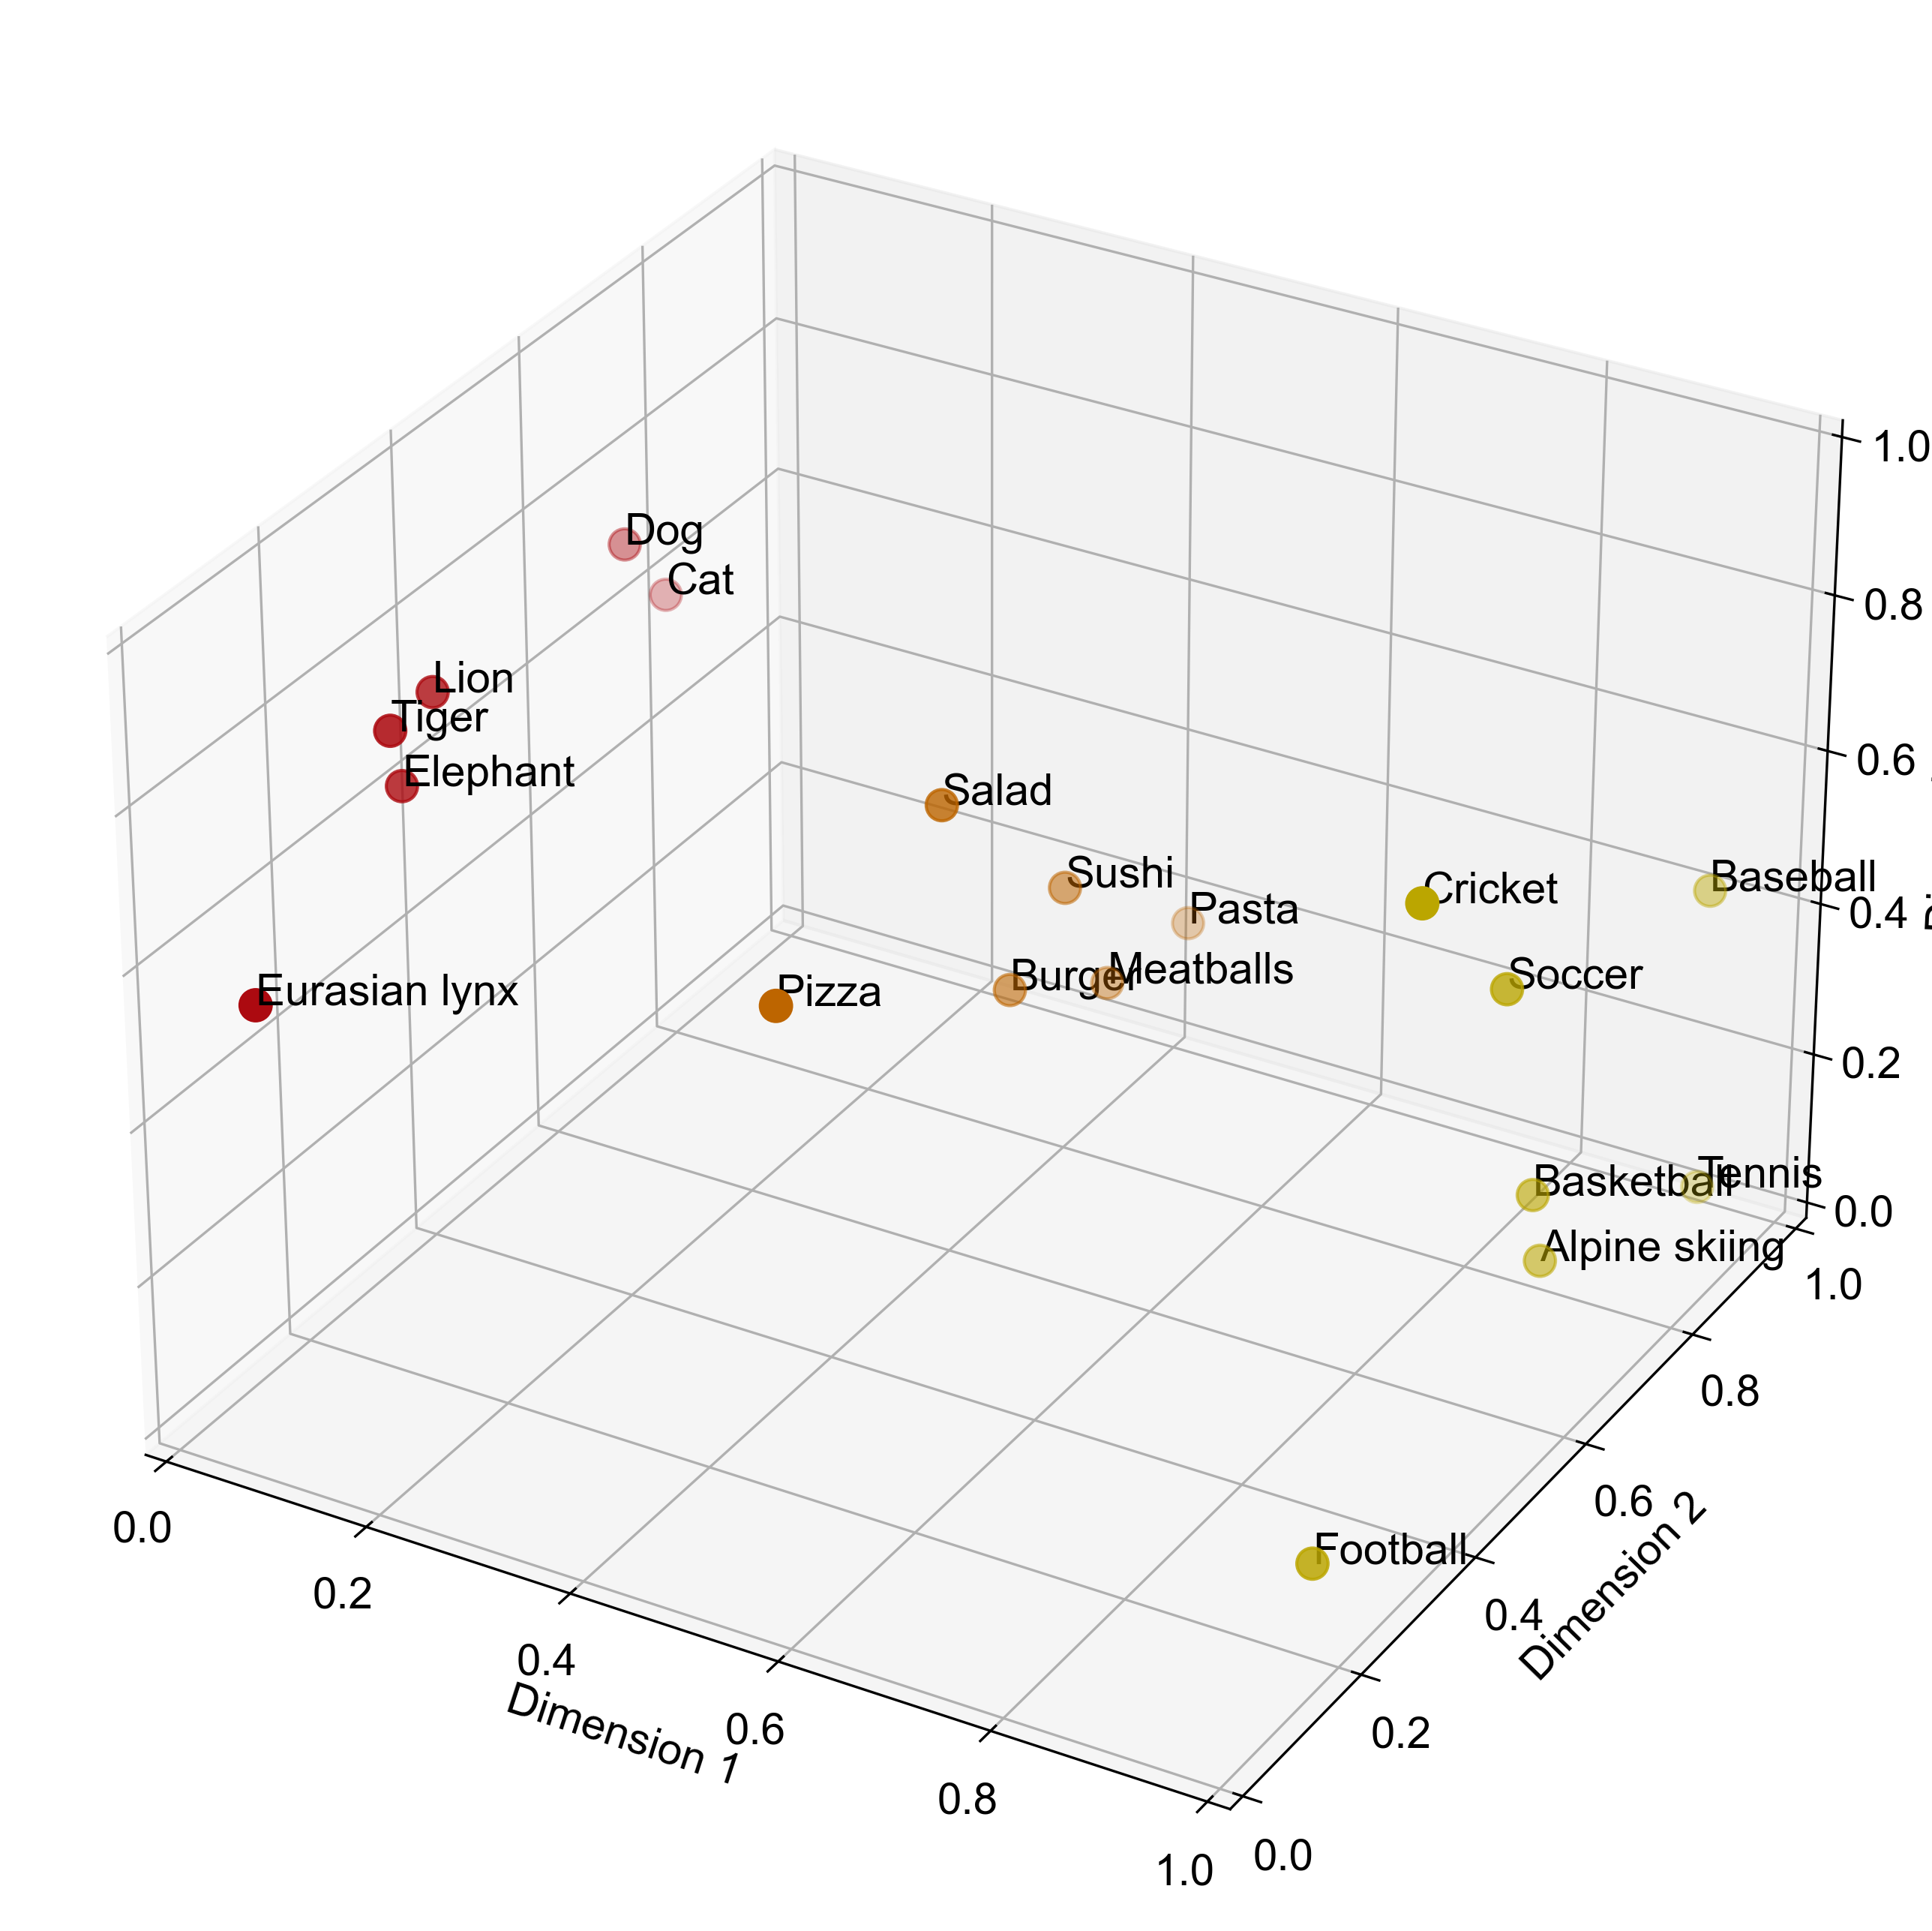
\includegraphics[width=\textwidth]{content/figures/assets/04-background-word-plot.png}
    \caption{Simplified 3D space with simplified embeddings for various words}
    \label{fig:background_word_plot}
\end{figure}



There are numerous types of models and techniques that have been developed to efficiently compute vector embeddings. One such is \gls{CBOW} and Skip-gram models, introduced by Mikolov et al. \cite{mikolov_efficient_2013}. These were early yet foundational methods for generating word embeddings. These models leverage large corpora to predict tokens from their context (CBOW), or with the context from the tokens (Skip-gram). Both of these techniques leverage the trained models ability to learn semantic and syntactic nuances of the tokens in the training corpus \cite{mikolov_efficient_2013, mikolov_distributed_2013}.


Advancements in vector embedding technologies enhance \gls{NLP} tasks such as text classification and sentiment analysis. Embedding models that can process language or images with nuance and precision are crucial for accurate real-world applications \cite{pennington_glove_2014}.


There are new Embedding functions released often, built-upon different language models and employing various different techniques. The evaluation of these embedding functions often remains constrained to a narrow set of tasks. Muennighoff et al. \cite{muennighoff_mteb_2023} tried to address this issue by introducing \gls{MTEB}, which spans 8 embedding tasks covering a total of 58 datasets and 112 languages. The leaderboard is currently actively maintained on hunggingface \footnote{\href{https://huggingface.co/spaces/mteb/leaderboard}{Massive Text Embedding Benchmark (MTEB) Leaderboard on Huggingface}}.


Two models that rank highly on the leaderboard is Salesforce's open source \textit{SFR-Embedding-Mistral} model which exemplifies advancements in embedding technology for text retrieval tasks \cite{meng_sfr-embedding-mistral_2024}. Similarly, OpenAI has developed several closed source embedding models that also rank highly on the MTEB leaderboard \cite{openai_new_2024, openai_new_2024-1}.


Embeddings are often used to compare documents against each other, or against a given user query. This is often done by computing similarity scores between words, phrases, or documents, which are represented as vectors in the embedding space. These scores quantify the closeness, or "similarity" between different texts.


The similarity between two vector representations is typically measured using the cosine similarity metric. This calculates the cosine of the angle between two vectors. This metric ranges from -1 (the exact opposite document) to 1 (the exact same document), with 0 indicating orthogonality (no similarity). The cosine similarity \( \text{sim}(u, v) \) between two vectors \( u \) and \( v \) is defined as:


\begin{equation}
\text{sim}(u, v) = \frac{u \cdot v}{\|u\| \|v\|}
\end{equation}


where \( u \cdot v \) is the dot product of the vectors \( u \) and \( v \), and \( \|u\| \) and \( \|v\| \) are the Euclidean norms of both vectors.


\section{RAG}


\gls{RAG} is the process of integrating retrieval mechanisms into the generative models. This approach effectively combines the strengths of both retrieval and generative language modelling to enhance a model's ability to accurately recall factual information by utilising an external knowledge base during the generation process \cite{lewis_retrieval-augmented_2021}.


\gls{RAG} was developed to address the limitations of large pre-trained language models that could compress a large training corpus into its weights, but could struggle with accessing and precisely manipulating this information when required. The term "hallucination" would come to describe the event where models would "recall" incorrect information, as shown in figure ~\ref{fig:hallucination_example}.


\begin{figure}[H]
\centering
\begin{tikzpicture}
    \newlength{\boxwidth}
    \setlength{\boxwidth}{0.4\textwidth}

    \node[draw, rectangle, rounded corners=2pt, inner sep=5pt, text width=\boxwidth, align=center] (a) {
        \smaller{What was the name of the spacecraft that took the first humans to Mars?}
    };
    \node[draw, rectangle, rounded corners=2pt, inner sep=5pt, text width=\boxwidth, align=center, right=of a, xshift=0.5cm] (b) {
        \smaller{The first humans were taken to Mars by the spacecraft Ares I, which landed on the Martian surface in 2025.}
    };

    \draw[-latex, line width=1mm] (a) -- (b);

    \node[align=center, below=0.1cm of a] (c) {\footnotesize Input};
    \node[align=center, below=0.1cm of b] (d) {\footnotesize Model output};
\end{tikzpicture}
\caption{An example of how a model can hallucinate an answer to a question.}
\label{fig:hallucination_example}
\end{figure}



The fact that language models tend to have a propensity to hallucinate, and the simple fact that it is very time consuming to train language models, mean these models would often lag behind in knowledge-intensive applications where correctness is crucial. The integration of a non-parametric memory, or an external knowledge base, allows these models to retrieve relevant information during the generation process and thereby producing more accurate responses \cite{lewis_retrieval-augmented_2021}.


In a typical \gls{RAG} setup, the systems architecture is split into two main components: the retriever and the generator. The retriever is a language model trained to search and fetch relevant documents. Nowadays, this process often utilises dense vector representations of documents (see section ~\ref{sec:embedding_functions}) which enables efficient and effective search \cite{guu_realm_2020}.


The returned documents are then fed into the generator, this is a \gls{seq2seq} model, which then synthesises the information into coherent text. The generator is often instructed to only use authoritative facts that are returned from the retriever and not rely on its internal knowledge for factual statements. This dual-component approach allows \gls{RAG} to dynamically access a large corpus of knowledge while maintaining its ability to generate fluent and contextually appropriate language \cite{lewis_retrieval-augmented_2021}. This method has shown significant improvement over a purely parametric-approach in various tasks such as question answering and fact verification \cite{brown_language_2020, sachan_end--end_2021}.


When google announced Gemini 1.5 \cite{gemini_team_gemini_2024} they claimed it could effectively recall knowledge over prompts as large as a million tokens. It remains to be seen if the hallucination, training-time and context length problems can be overcomed and remove the need for a \gls{RAG} system when building knowledge-intensive applications on-top of a \gls{LLM}.


\section{AI Assistants}


AI assistants is a type of AI-system that is designed to support human users by performing tasks that typically require human intelligence. Stuart Russell and Peter Norvig wrote in \textit{Artificial Intelligence: A Modern Approach} that an assistant should interact with their environment to achieve specific goals rationally and effectively \cite{russell_artificial_2016}.


AI assistants must be good at \gls{NLP} for effective communication with humans in addition to good knowledge representation such as with a \gls{RAG} toolchain. The assistant must also possess good reasoning and decision-making abilities, as those exhibited by a modern \gls{LLM}. An assistant should also utilise machine learning to improve from user interactions.


\section{Measuring usability and acceptance of new technologies}


To assess how effectively a user can interact with a technology, for instance, an AI assistant, Jakob Nielsen's "Usability Engineering" \cite{nielsen_chapter_1993-1} is a seminal book that defines usability in terms of learnability, efficiency, memorability, safety, and satisfaction. All of these can be measured through specific metrics. The IBM Computer Usability Satisfaction Questionnaires, developed by Lewis \cite{lewis_ibm_1995}, offer a tool that’s been validated through the years to measure these dimensions.


Interactions with AI agents through conversation is very affected by the agent's ability to engage in social dialogue. Bickmore and Cassell \cite{bickmore_social_2005} discuss the importance of dialogue in building engagement long-term between users and conversational agents. Their conversational agents communicated over the phone, but their framework for understanding the qualitative feedback from users about their experiences can also be applied with an AI assistant.


\gls{TAM} was introduced by Davis \cite{davis_perceived_1989} and is particularly relevant for examining the acceptance of new technologies such as AI assistants. \gls{TAM} suggests that perceived usefulness and ease of use are key factors for whether a new technology is accepted and used. The model is useful for investigating users' attitudes towards the utility and usability of new technologies, not the least of which is AI and AI assistants.


\gls{ECM} was introduced by Bhattacherjee \cite{bhattacherjee_understanding_2001} in 2001 and it extends the understanding of user satisfaction beyond initial acceptance which is outlined in \gls{TAM}. \gls{ECM} includes user expectations, perceived performance, and confirmation of expectations into the satisfaction assessment. This model is especially useful in assessing whether a technology meets or exceeds the users' expectations over time.


\section{Related work area}


% \sweExpl{Relaterade arbeten}


...




\subsection{Major related work 1}


Carrier clouds have been suggested as a way to reduce the delay between the users and the cloud server that is providing them with content. However, there is a question of how to find the available resources in such a carrier cloud. One approach has been to disseminate resource information using an extension to OSPF-TE, see Roozbeh, Sefidcon, and Maguire \cite{roozbeh_resource_2013}.


\subsection{Major related work n}


\subsection{Minor related work 1}


...


\subsection{Minor related work n}


\section{Summary}


% \sweExpl{Det är trevligt om detta kapitel
%   avslutas med en sammanfattning. Till exempel kan du inkludera en tabell som
%   sammanfattar andras idéer och fördelar och nackdelar med varje - så som
%   senare kan du jämföra din lösning till var och en av dessa. Detta kommer
%   också att hjälpa dig att definiera de variabler som du kommer att använda
%   för din utvärdering.}


% \engExpl{It is nice to have this chapter conclude with a summary. For
%   example, you can include a table that summarizes other people's ideas and
%   benefits and drawbacks with each - so as later you can compare your solution
%   to each of them. This will also help you define the variables that you will
%   use for your evaluation.}


\cleardoublepage